\documentclass[11pt,a4paper]{article}

\usepackage{../../templates/style}

\begin{document}

\begin{problem}{หุ่นยนต์ 1000S}{standard input}{standard output}{1 second}{32 megabytes}


หุ่นยนต์รุ่น \textit{1000S} สามารถเดินไปมาบนระนาบสองมิติ  หุ่นยนต์รุ่น \textit{1000S} นี้จะรับชุดคำสั่งให้เดินไปในทิศทางต่าง ๆ  โดยชุดคำสั่งจะประกอบด้วยคำสั่งที่ระบุทิศทางเหนือ ใต้ ตะวันออก และตะวันตก ซึ่งระบุด้วยอักษร \textbf{N S E }และ \textbf{W} ตามลำดับ สำหรับแต่ละคำสั่ง หุ่นยนต์จะเคลื่อนไปในทิศทางที่ระบุในคำสั่งเป็นระยะหนึ่งหน่วย

พิจารณาตัวอย่างชุดคำสั่ง \textbf{NNEESW} สำหรับชุดคำสั่งดังกล่าว หุ่นยนต์ที่เริ่มต้นเคลื่อนที่จากตำแหน่ง $(0,0)$ จะเดินในลักษณะตามรูปด้านล่าง

\begin{figure}[!h]
\centering
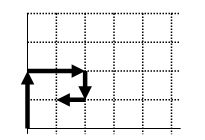
\includegraphics[width=0.4\textwidth]{../latex/img/1167/1167-1.png}
\end{figure}
หุ่นยนต์จะมีตำแหน่งสุดท้ายป็นตำแหน่ง $(1,1)$

                ในการสั่งงานหุ่นยนต์รุ่น \textit{1000S} ตัวหนึ่งผ่านทางการส่งสัญญาณไมโครเวฟ พบว่าในการส่งชุดคำสั่งมีคำสั่งที่หายไป $K$ คำสั่ง  ทำให้ไม่มีใครทราบอย่างแน่นอนว่าหุ่นตัวดังกล่าวอยู่ที่จุดใดในแผนที่

                พิจารณาตัวอย่างชุดคำสั่ง \textbf{NNEESW} ที่มีคำสั่งหายไป $2$ คำสั่ง  ด้านล่างแสดงตำแหน่งสุดท้ายที่เป็นไปได้ทั้งหมดของหุ่นยนต์ดังกล่าว

\begin{figure}[!h]
\centering
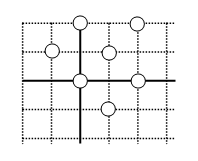
\includegraphics[width=0.4\textwidth]{../latex/img/1167/1167-2.png}
\end{figure}


ทางทีมงานจะต้องใช้เรดาห์เพื่อหาว่าหุ่นดังกล่าวอยู่ที่ตำแหน่งใด  และจะส่งหุ่นรุ่น \textit{1000S} อีกตัวให้เดินทางจากจุด $(0,0)$ เพื่อขนหุ่นตัวแรกกลับมาที่จุด $(0,0)$

อย่างไรก็ตาม หุ่นรุ่น \textit{1000S} ตัวที่สองจะต้องเติมพลังงานเสียก่อน โดยพลังงานที่ใช้จะต้องเพียงพอที่จะเคลื่อนที่ไปและกลับจากตำแหน่งของหุ่นตัวแรกได้   หุ่นรุ่น \textit{1000S} จะใช้พลังงาน $1$ หน่วยในการเคลื่อนที่ในระยะ $1$ หน่วย   คุณมีหน้าที่เติมพลังงานให้กับหุ่นให้เพียงพอที่จะดำเนินการดังกล่าว แม้ว่าตอนนี้จะยังไม่ทราบตำแหน่งที่แน่นอนของหุ่นตัวแรกก็ตาม

จากตัวอย่างข้างต้น หุ่นตัวที่สองอาจจะต้องเดินทางไปจนถึงตำแหน่ง $(2,2)$ และเดินกลับ ซึ่งต้องเคลื่อนที่ทั้งสิ้น $8$ หน่วย ดังนั้นคุณต้องเติมพลังงานอย่างน้อย $8$ หน่วยให้กับหุ่นยนต์

\bigskip
\underline{\textbf{โจทย์}}  จงเขียนโปรแกรมรับชุดคำสั่งของหุ่นยนต์รุ่น \textit{1000S} ตัวแรกที่เริ่มเคลื่อนที่จากจุด $(0,0)$ และจำนวนเต็ม $K$ ที่ แทนจำนวนคำสั่งที่หายไป จากนั้นคำนวณหาว่าจะต้องเติมพลังงานน้อยที่สุดกี่หน่วยให้กับหุ่นยนต์ตัวที่สองที่มากพอที่จะเดินทางจากจุดเริ่มต้นไปกู้ซากหุ่นตัวแรกแล้วเดินกลับมาที่จุดเริ่มต้นได้


\InputFile

\textbf{บรรทัดแรก} ระบุชุดคำสั่งสำหรับหุ่นยนต์รุ่น \textit{1000S} ชุดคำสั่งนี้จะเป็นสตริงความยาวไม่เกิน $100$ ตัวอักษร และจะประกอบไปด้วยตัวอักษร N S E และ W เท่านั้น  

\textbf{บรรทัดที่สอง} ระบุจำนวนเต็ม $K$ ที่มีค่าไม่มากกว่าความยาวของสตริงแทนชุดคำสั่งในบรรทัดแรก


\OutputFile

\textbf{มีบรรทัดเดียว} ประกอบไปด้วยจำนวนเต็มระบุระดับพลังงานที่น้อยที่สุดที่ต้องเติมให้กับหุ่นยนต์ตัวที่สอง


\Examples

\begin{example}
\exmp{NNEESW
2}{8}%
\exmp{NE
2}{0}%
\exmp{NWSSSSE
1}{8}%
\end{example}


\Source

 IOI Thailand League 2010 เดือนมีนาคม

\end{problem}

\end{document}